\section{Connectivity}


The human brain is factually a giant network of functionally specialized units connected by dynamically configurable communication pathways. In the last decade, researchers have increasingly and successfully turned to graph analysis to unveil activated brain networks and to describe their non-trivial topological properties in a compact and objective way (Fallani et al., 2014) such as in the case of language comprehension (Chai et al., 2016). 

Graph analysis also aided in our understanding of the dysfunctional brain. There is growing evidence that Alzheimer's disease, schizophrenia, etc., relate to deviations in graph theoretical properties commonly found in healthy subjects, such as small-worldness, rich club hubs and community structures, that could serve as biomarkers for diagnosis and rehabilitation (Stam and Reijneveld, 2007).

B issues such as comparing graphs with differently defined thresholds and optimal network sizes (Wijk et al., 2010), the main challenge with graph analysis is to account for the brain's dynamicity at different frequency, temporal, and spatial scales. Dynamic and multilayers networks have been recently introduced to account esides traditional for the brain's inherently dynamic processes (Domenico, 2017).

Albeit graph analysis has gained popularity in neuroscience, for some critics it has not yet proceeded beyond the exploratory stage: is it only for comparing networks across paradigms, subject groups and tasks? Most certainly, graph analysis has the ability to go beyond such scenarios and to uncover the dynamic information flow underlying cognitive functioning. 

A specific cognitive procedure could come with constraints that in turn can be used to rule out alternative pathways, such as different anatomical routes connecting areas (fiber tracts), the speed of information transfer along them, and the energy consumption that comes with the information flow. This is, basically, what Deslauriers-Gauthier and co-workers at INRIA did after using diffusion MRI data as a basis of the connections of their Bayesian network model: they added functional constraints in terms of information velocity between nodes.

An interesting starting point is the event related potential (ERP), a characteristic amplitude deflection of an EEG-, intracranial- or even intracellular signal evoked by, and in synchrony with, a meaningful external stimulus (Luck, 2005). Correlations between ERPs and behavioral measures are easily demonstrated but their lack of sensitivity and specificity impede their use as the sole biomarker for diagnosis and rehabilitation, unless their physiological origin is clear (Rennie et al., 2002).

Neural mass models have been shown to replicate ERPs in terms of excitatory and inhibitory neural populations, range-dependent connections, dendritic delays, and nonlinear response functions (David et al., 2005). Compared to the graph-theoretical models they are very realistic but the flipside is that they are too complex to be used for examining the impact of biological and organizational constraints that could narrow down the search for a dynamic network solution across temporal and spatial scales.

Little is known about the signature networks of ERPs (De Munck and Bijma, 2010) but graph theory could be used to gauge the time- and energy efficiency of the information flow through alternative graphs, to compare the predicted ERPs with experimentally recorded ones, and to judge whether some graph components are wrong, missing or irrelevant. In summary, graph analysis holds sufficient, yet unexplored potential to investigate the structure-function interplays and dynamic routing of functional interactions on the anatomical connectivity so as to evaluate and validate the mechanisms that shape ERPs (Griffa et al., 2017). When successful, it could also add to our nderstanding of the dysfunctional brain and even be used to monitor the efficiency of rehabilitation programs.

Neural mass models have been shown to replicate ERPs in terms of excitatory and inhibitory neural populations, range-dependent connections, dendritic delays, and nonlinear response functions (David et al., 2005). Compared to the graph-theoretical models they are very realistic but the flipside is that they are too complex to be used for examining the impact of biological and organizational constraints that could narrow down the search for a dynamic network solution across temporal and spatial scales.

Little is known about the signature networks of ERPs (De Munck and Bijma, 2010) but graph theory could be used to gauge the time- and energy efficiency of the information flow through alternative graphs, to compare the predicted ERPs with experimentally recorded ones, and to judge whether some graph components are wrong, missing or irrelevant. In summary, graph analysis holds sufficient, yet unexplored potential to investigate the structure-function interplays and dynamic routing of functional interactions on the anatomical connectivity so as to evaluate and validate the mechanisms that shape ERPs (Griffa et al., 2017). When successful, it could also add to our nderstanding of the dysfunctional brain and even be used to monitor the efficiency of rehabilitation programs.

Neural mass models have been shown to replicate ERPs in terms of excitatory and inhibitory neural populations, range-dependent connections, dendritic delays, and nonlinear response functions (David et al., 2005). Compared to the graph-theoretical models they are very realistic but the flipside is that they are too complex to be used for examining the impact of biological and organizational constraints that could narrow down the search for a dynamic network solution across temporal and spatial scales.

Little is known about the signature networks of ERPs (De Munck and Bijma, 2010) but graph theory could be used to gauge the time- and energy efficiency of the information flow through alternative graphs, to compare the predicted ERPs with experimentally recorded ones, and to judge whether some graph components are wrong, missing or irrelevant. In summary, graph analysis holds sufficient, yet unexplored potential to investigate the structure-function interplays and dynamic routing of functional interactions on the anatomical connectivity so as to evaluate and validate the mechanisms that shape ERPs (Griffa et al., 2017). When successful, it could also add to our nderstanding of the dysfunctional brain and even be used to monitor the efficiency of rehabilitation programs.

\section{Volume Conduction}

The head volume conductor model is quite interesting. The brain conducts electrical activity, this is how the electrical activity can be measured on the scalp. Volume conduction refers to this process of conducting electrical activity through a medium. 

Figure~\ref{conduction} shows several problems that the reverse problem has to deal with. In situation A, there would be no problem. In this situation, every EEG electrode measures one and only one electrical source within the brain. However, this is not what happens in reality. 

\begin{figure}[!htb]
\caption{Volume Conduction \cite{cohen2014analyzing}.}
\label{conduction}
    \centering
    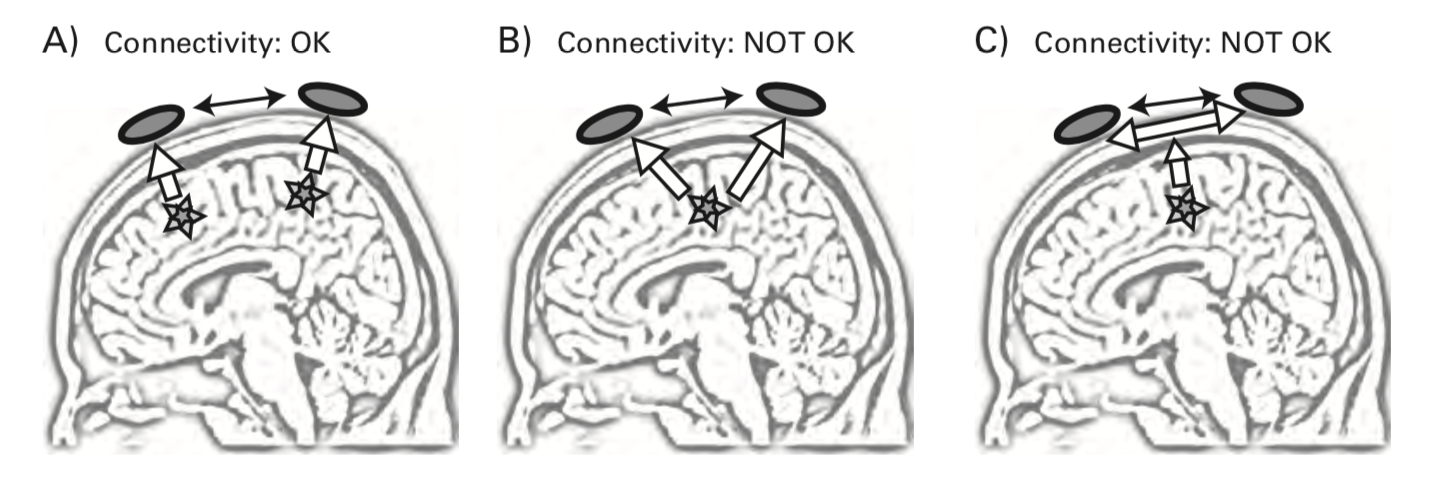
\includegraphics[width=\textwidth]{fig/conduction}
\end{figure}

Reality is a combination of situations B and C. Situation B shows that electrical sources in the brain generate large electromagnetic fields which are recorded by more than one EEG electrode. Situation C shows that the scalp also conducts electricity. These two situations have a big effect on connectivity measures.
